\documentclass[10pt,a4paper]{article}
\usepackage[margin=1.8cm]{geometry}
\usepackage{newtxtext,newtxmath}
\usepackage{booktabs,tabularx,graphicx,subcaption,float,microtype}
\usepackage[colorlinks=true,allcolors=blue]{hyperref}
\newcommand{\mf}{\ensuremath{\mathrm{macro\text{-}F1}}}
\newcommand{\ci}{95\% CI}
\title{Supplementary Material\\\large Controlled Component Comparisons and Cross-Cohort Failure Analysis for Single-Channel EEG Sleep Staging}
\author{Ngo Nhat Quan and Pham Thai Son}
\date{}

\begin{document}
\maketitle

This supplement contains implementation details and descriptive tables moved from the main manuscript.
The evidence labels are unchanged: seed 42 is primary, seed 123 is a post-protocol sensitivity repeat,
SHHS1 E1/E2 analyses are secondary on an opened cohort, and SHHS1 E3--E2/E4 analyses are post-hoc.
E6 estimates mean and standard deviation from each complete unlabelled target recording; it is label-free
but transductive at recording level, not purely inductive zero-shot inference.

\section*{Supplementary Methods S1: model and training details}

The control encoder contains 15 CNN branches: three context groups (current, previous and next; C/P/N)
crossed with five stage-specific detectors. Each branch uses two convolutional blocks and a small head;
their outputs form a 75-dimensional feature vector. The ResNet-1D encoder uses a convolutional stem,
three residual blocks and global average pooling to produce a 128-dimensional representation from the
current epoch only. Thus, E1--E0 isolates the sequence-model substitution, whereas E2--E1 replaces the
encoder, removes explicit P/N context and changes feature dimension.

The TCN projects inputs to 128 dimensions and uses six residual blocks with dilations 1, 2, 4, 8, 16
and 32, symmetric padding and dropout 0.2, giving a 253-epoch receptive field. The BiLSTM has 128 hidden
units per direction. Encoders are fitted first, selected on validation data, hash-verified and used to
cache features without gradients; sequence models are then fitted on these frozen caches. CNN and
BiLSTM optimisation uses Adam; ResNet-1D uses AdamW; TCN uses Adam. Exact learning rates are $10^{-3}$,
$10^{-2}$, $10^{-3}$ and $5\times10^{-4}$, respectively. Batch sizes are 64 epochs for encoders, four
recordings for BiLSTM and eight recordings for TCN. No label smoothing or data augmentation is used.

\section*{Supplementary results}

\begin{table}[H]
\centering\small
\caption{S1. Per-class Sleep-EDF metrics for E3 and E6 (seed 42).}
\begin{tabular}{lrrrrrrr}
\toprule
Stage & E3 Prec. & E3 Rec. & E3 F1 & E6 Prec. & E6 Rec. & E6 F1 & $\Delta$F1 \\
\midrule
W & .9338 & .9271 & .9304 & .9391 & .9169 & .9279 & +.0026 \\
N1 & .5149 & .5410 & .5276 & .5032 & .5219 & .5124 & +.0152 \\
N2 & .8583 & .8447 & .8514 & .8401 & .8368 & .8385 & +.0130 \\
N3 & .8072 & .8097 & .8085 & .7160 & .7779 & .7457 & +.0628 \\
REM & .8274 & .8413 & .8343 & .8227 & .8197 & .8212 & +.0131 \\
\bottomrule
\end{tabular}
\end{table}

\begin{table}[H]
\centering\small
\caption{S2. Pooled E3 confusion matrix on Sleep-EDF (rows: reference; columns: prediction).}
\begin{tabular}{lrrrrr}
\toprule
 & W & N1 & N2 & N3 & REM \\
\midrule
W & 61{,}133 & 3{,}888 & 416 & 56 & 448 \\
N1 & 3{,}283 & 11{,}643 & 4{,}867 & 105 & 1{,}624 \\
N2 & 539 & 5{,}496 & 58{,}394 & 2{,}271 & 2{,}432 \\
N3 & 30 & 45 & 2{,}377 & 10{,}558 & 29 \\
REM & 483 & 1{,}542 & 1{,}984 & 90 & 21{,}736 \\
\bottomrule
\end{tabular}
\end{table}

\begin{table}[H]
\centering\small
\caption{S3. Sleep-EDF \mf\ under two fixed seeds.}
\begin{tabular}{lrrr}
\toprule
Configuration & Seed 42 & Seed 123 & Difference \\
\midrule
E0 & .7754 & .7755 & +.0000 \\
E1 & .7802 & .7776 & -.0026 \\
E2 & .7835 & .7828 & -.0007 \\
E3 & .7904 & .7883 & -.0022 \\
E4 & .7891 & .7887 & -.0004 \\
E6 & .7691 & .7780 & +.0089 \\
\bottomrule
\end{tabular}
\end{table}

\begin{table}[H]
\centering\small
\caption{S4. Seed sensitivity of pre-specified Sleep-EDF contrasts; Holm correction is within seed.}
\resizebox{\textwidth}{!}{\begin{tabular}{lll}
\toprule
Contrast & Seed 42: $\Delta$ [\ci], $p_{\rm Holm}$ & Seed 123: $\Delta$ [\ci], $p_{\rm Holm}$ \\
\midrule
E1--E0 & .004811 [$-.000915$, .010193], .1022 & .002188 [$-.002870$, .007043], .9130 \\
E2--E1 & .003251 [$-.002370$, .008808], .1036 & .005143 [$-.000571$, .011292], .2400 \\
E3--E2 & .006962 [.000305, .014520], .8989 & .005478 [$-.002611$, .015796], .9130 \\
E3--E6 & .021319 [.012179, .030698], .0012 & .010249 [.002435, .017989], .1313 \\
\bottomrule
\end{tabular}}
\end{table}

\begin{table}[H]
\centering\small
\caption{S5. Seed-123 wall-clock training and validation time (10 folds, sequential, same GPU).}
\begin{tabular}{lrr}
\toprule
Configuration & Total & Mean per fold \\
\midrule
E0: 15-CNN + BiLSTM & 33 h 35 min 36 s & 3 h 21 min 34 s \\
E1: 15-CNN + TCN & 14 min 17 s & 1 min 26 s \\
E2: ResNet-1D + TCN & 2 h 44 min 57 s & 16 min 30 s \\
E3: fixed scale & 3 h 16 min 40 s & 19 min 40 s \\
E4: band-pass & 2 h 55 min 56 s & 17 min 36 s \\
E6: target-record $z$-score & 2 h 24 min 44 s & 14 min 28 s \\
\bottomrule
\end{tabular}
\end{table}

\begin{table}[H]
\centering\small
\caption{S6. Seed-123 sensitivity on the same 180 SHHS1 participants.}
\resizebox{\textwidth}{!}{\begin{tabular}{lrrrr}
\toprule
ID & Subject-mean \mf & Pooled \mf & Accuracy & $\kappa$ \\
\midrule
E0 & .5303 & .5785 & .6738 & .5420 \\
E2 & .5409 & .5858 & .6874 & .5597 \\
E3 & .5634 & .6031 & .7003 & .5772 \\
E4 & .5732 & .6147 & .7064 & .5869 \\
E6 & .5503 & .5865 & .6873 & .5552 \\
\bottomrule
\end{tabular}}
\end{table}

\begin{table}[H]
\centering\small
\caption{S7. Per-class transfer of E3; Pred/True is a marginal emission ratio, not calibration.}
\resizebox{\textwidth}{!}{\begin{tabular}{lrrrrrrr}
\toprule
& \multicolumn{2}{c}{Sleep-EDF} & \multicolumn{4}{c}{SHHS1} & \\
Stage & F1 & Pred/True & Prec. & Rec. & F1 & Pred/True & $\Delta$F1 \\
\midrule
W & .9304 & .993 & .8823 & .8014 & .8399 & .908 & -.0905 \\
N1 & .5276 & 1.051 & .2528 & .5437 & .3451 & 2.151 & -.1824 \\
N2 & .8514 & .984 & .7394 & .7349 & .7372 & .994 & -.1143 \\
N3 & .8085 & 1.003 & .9440 & .2582 & .4055 & .273 & -.4030 \\
REM & .8343 & 1.017 & .6052 & .8939 & .7218 & 1.477 & -.1125 \\
\bottomrule
\end{tabular}}
\end{table}

\begin{table}[H]
\centering\small
\caption{S8. Pooled E3 confusion matrix on SHHS1 (rows: reference; columns: prediction).}
\begin{tabular}{lrrrrr}
\toprule
 & W & N1 & N2 & N3 & REM \\
\midrule
W & 29{,}638 & 4{,}481 & 1{,}171 & 21 & 1{,}672 \\
N1 & 874 & 3{,}807 & 601 & 3 & 1{,}717 \\
N2 & 2{,}348 & 5{,}947 & 56{,}063 & 324 & 11{,}605 \\
N3 & 78 & 39 & 16{,}674 & 5{,}888 & 127 \\
REM & 655 & 784 & 1{,}311 & 1 & 23{,}183 \\
\bottomrule
\end{tabular}
\end{table}

\begin{table}[H]
\centering\small
\caption{S9. Per-class SHHS1 metrics for E3 and E2.}
\resizebox{\textwidth}{!}{\begin{tabular}{lrrrrrrr}
\toprule
Stage & E3 Prec. & E3 Rec. & E3 F1 & E2 Prec. & E2 Rec. & E2 F1 & $\Delta$F1 \\
\midrule
W & .8823 & .8014 & .8399 & .8780 & .7275 & .7957 & +.0442 \\
N1 & .2528 & .5437 & .3451 & .2367 & .3528 & .2833 & +.0618 \\
N2 & .7394 & .7349 & .7372 & .7362 & .6937 & .7143 & +.0228 \\
N3 & .9440 & .2582 & .4055 & .9659 & .2496 & .3967 & +.0087 \\
REM & .6052 & .8939 & .7218 & .4886 & .9450 & .6442 & +.0776 \\
\bottomrule
\end{tabular}}
\end{table}

\begin{table}[H]
\centering\small
\caption{S10. Oracle prioritisation on E3 predictions. Values are potential leverage, not achievable performance.}
\begin{tabular}{lrr}
\toprule
Condition & \mf & Numerical gap recovered \\
\midrule
Observed E3 on SHHS1 & .6099 & --- \\
Correct N3$\rightarrow$N2 only & .7444 & .1345 (74.5\%) \\
Correct N2$\rightarrow$REM only & .6596 & .0497 (27.5\%) \\
E3 on Sleep-EDF & .7904 & --- \\
\bottomrule
\end{tabular}
\end{table}

\begin{table}[H]
\centering\small
\caption{S11. Post-hoc reference-label boundary and stable-interior diagnostic (seed 42).}
\begin{tabular}{llrrrr}
\toprule
Cohort & ID & Boundary \mf & Stable \mf & Boundary N3 recall & Stable N3 recall \\
\midrule
Sleep-EDF & E0 & .6179 & .8175 & .6121 & .9216 \\
Sleep-EDF & E3 & .6321 & .8346 & .6326 & .9316 \\
SHHS1 & E0 & .4323 & .5959 & .0633 & .4008 \\
SHHS1 & E3 & .4689 & .6220 & .0733 & .3900 \\
\bottomrule
\end{tabular}
\end{table}

E6 N3 recall is 0.2005 overall and 0.0721 in the same SHHS1 boundary neighbourhood, compared with
0.2582 and 0.0733 for E3. These regions use reference labels on both sides and are offline diagnostics,
not physiological transitions or deployable detectors.

\section*{Supplementary analyses: representation and context}

The mean silhouette coefficient is 0.2126 (SD 0.0356) for E1 and 0.1048 (SD 0.0229) for E2. This
comparison is descriptive: E1 consists of 75 class-posterior features, whereas E2 is an unconstrained
128-dimensional representation, so silhouette is not a like-for-like measure of downstream utility.

\begin{table}[H]
\centering\small
\caption{S12. Context-group ablation within E1.}
\begin{tabular}{lrrrrr}
\toprule
Condition & Overall \mf & $\Delta$ vs C & Boundary \mf & $\Delta$ vs C & N1 F1 \\
\midrule
C & .777477 & --- & .619102 & --- & .5011 \\
CP & .777733 & +.000257 & .617686 & -.001416 & .5022 \\
CN & .781585 & +.004108 & .618895 & -.000207 & .5055 \\
CPN & .780230 & +.002753 & .620055 & +.000953 & .5115 \\
\bottomrule
\end{tabular}
\end{table}

For the pre-specified CPN--C boundary comparison, $\Delta\mf=0.000953$, \ci\
$[-0.004588,0.006568]$ and Holm $p=1.000$ (36/78 subjects improved). Secondary CPN--CP and CPN--CN
intervals also include zero with Holm $p=1.000$. The result does not show that temporal context or P/N
information is useless; it only finds no detectable marginal benefit for this encoding in E1.

\begin{figure}[H]
\centering
\begin{subfigure}{0.48\textwidth}
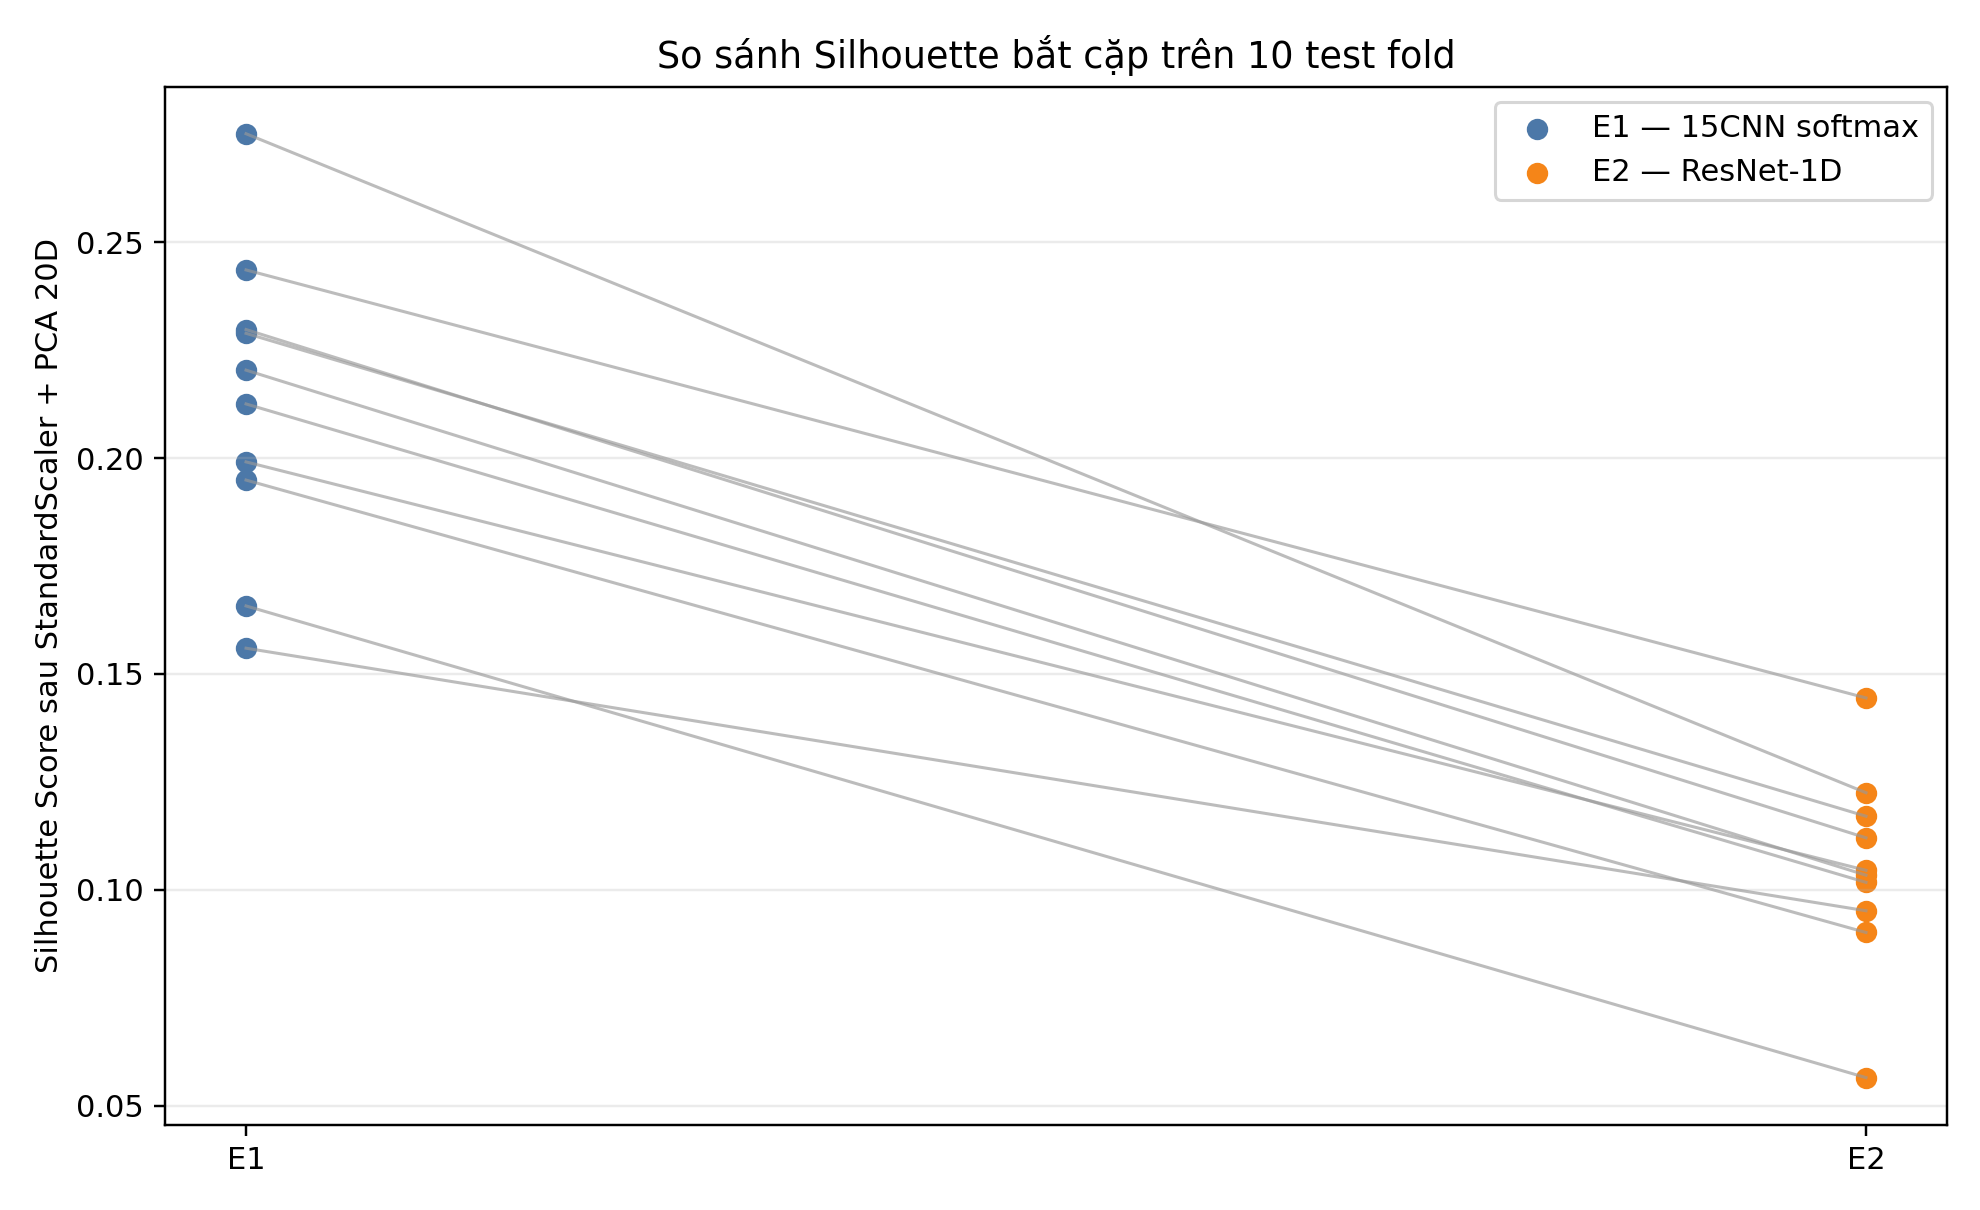
\includegraphics[width=\textwidth]{../figures/gate8_feature_silhouette.png}
\caption{Silhouette by fold.}
\end{subfigure}\hfill
\begin{subfigure}{0.48\textwidth}
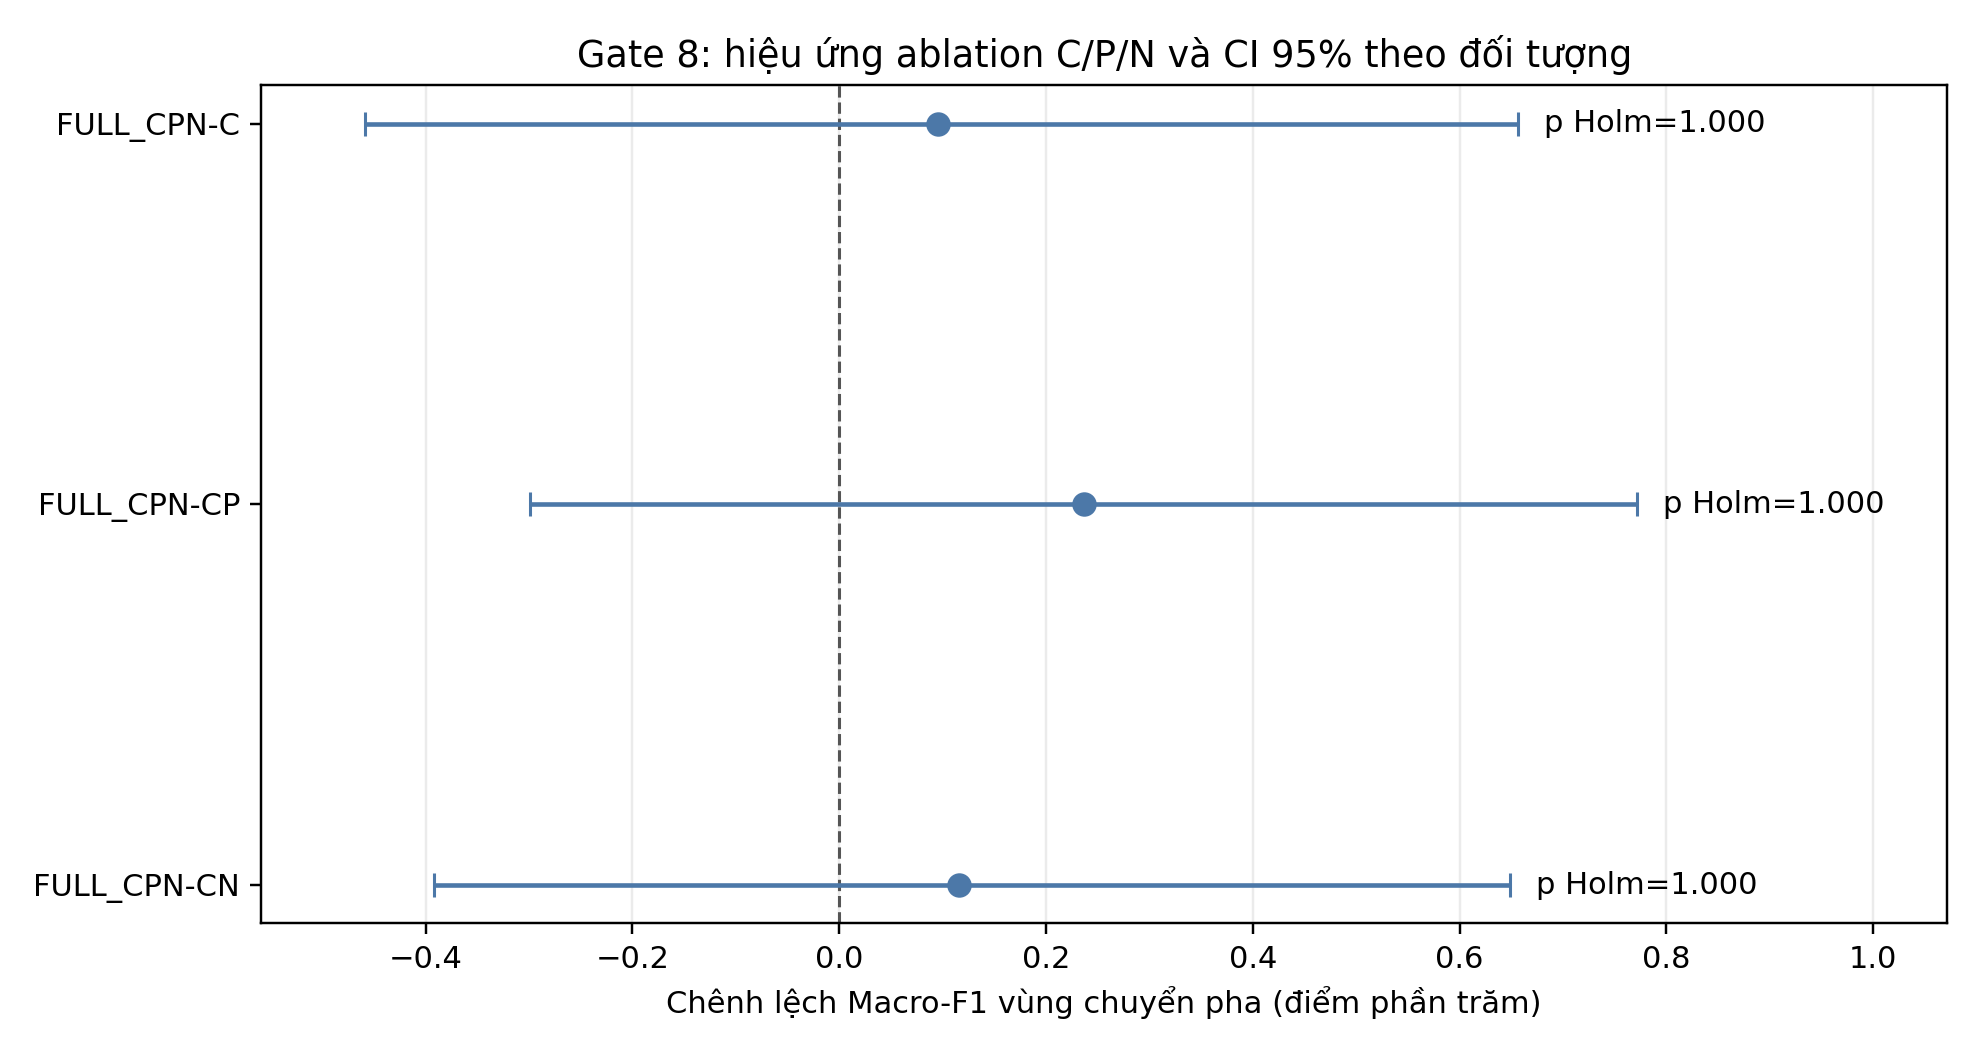
\includegraphics[width=\textwidth]{../figures/gate8_context_ablation_effects.png}
\caption{Context-ablation effects.}
\end{subfigure}
\caption{S1. Supporting representation and context analyses.}
\end{figure}

\section*{Provenance limitation}

Prediction artifacts and recomputed metrics are hash-verified. The SHHS run-manifest protocol hash
(`165d7cdf...fe93`) matches the retained historical snapshot \path{configs/shhs_zero_shot_v1.json}; the
currently checked-out \path{configs/shhs_v1_protocol.json} (`9541e233...fe9`) is an expanded post-run audit
record, not a replacement. The reconciliation is recorded in
\path{Reports/SHHS_PROTOCOL_PROVENANCE.md}.
This resolves the snapshot-level provenance discrepancy, while raw SHHS data and prediction artifacts
remain outside the repository and E6 remains a descriptive reanalysis of locked predictions.

\end{document}
